%        File: memoria.tex
%     Created: sáb jun 28 01:00  2008 C
% Last Change: sáb jun 28 01:00  2008 C
%
\documentclass[a4paper,spanish,12pt]{book}
\title{BLAS: Base Layer for Application Services}
\author{Eduardo Orive Vinuesa}
\usepackage{babel}
\usepackage{times}
\usepackage[T1]{fontenc}
\usepackage[utf8]{inputenc}
\usepackage[left=2.5cm, right=2.5cm]{geometry}
\usepackage{a4}
\usepackage{makeidx}
\usepackage{graphicx}
\usepackage{float}
\usepackage{url}
\usepackage{setspace}
\onehalfspacing
\usepackage{fancyheadings}
\usepackage{wrapfig}

\begin{document}
\tableofcontents

\maketitle

%cuerpo del documento


\chapter*{Introducción}
Actualmente casi la totalidad de las instalaciones inform\'aticas son redes, y una mayoria de estas est\'an conectadas a Internet o incluso la propia Internet forma parte de estas. 

Es en este entorno donde se desarrollan las arquitecturas de la mayor\'ia de los sistemas. Distribuidas y en una gran proporci\'on siguiendo el modelo Cliente-Servidor casi todas las nuevas aplicaciones o sistemas basan gran parte de su funcionalidad en la conectividad mediante redes. 

Sin embargo realizar aunque sea un prototipo de un servicio de red resulta caro en tiempo y no se obtienen resultados tangibles hasta que se han implementado una buena parte del codigo.
Tambi\'en muy com\'un ver que muchos prototipos sean descartados (total o parcialmente) y deban re-escribirse ya que, aunque su rendimiento sea aceptable, la seguridad que ofrecen no lo es, con lo que el proceso de crear el servicio duplica su coste cuando el sistema llega a la etapa de producci\'on.

No obstante la escritura de un servicio de Red puede reducirse considerablemente si se implementan tan solo las caracteristicas particulares de su protocolo. Basicamente cualquier protocolo puede entenderse como un automata m\'as o menos complejo, siguiendo este modo de dise\~{o} puede simplificarse de manera considerable el trabajo del programador.
Existen multitud de funcionalidades ligadas a los programas que ofrecen servicios TCP que consumen mucho tiempo y que normalmente su implementaci\'on resulta bastante repetitiva:
\begin{enumerate}
	\item Entrada controlada de datos.
	\item Registro (o registros) de actividad y error.
	\item Lectura de los archivos de configuraci\'on.
	\item Parseado de los parametros de arraque.
\end{enumerate}

\section{Historia de los servicios informáticos}
Despu\'es del desarrollo de la primera generación de computadoras el número de estas empezo a aumentar, aunque su disponibilidad estaba limitada a una unica unidad por cada entidad. Estas máquinas requerían de un entorno ambiental muy concreto y el acceso instalaciones donde se albergaban estaba severamente limitado. Por estas mismas limitaciones y para maximizar la disponibilidad se ideo un sistema limitado de terminales remotas, los teletipos, cuya funcion era comunicar con el ordenador central pudiendo utilizar enlaces dedicados o conmutados (lineas telefónicas), permitir la inserción de programas y recuperar el resultado una vez el sistema hubiera finalizado. Estos sistemas de comunicación y control remotos merecen la consideración de servicios informaticos.

Con el tiempo la versatilidad de los sistemas fue ampliandose, los ordenadores dejaron de emplearse como meras ejecutoras de algoritmos y empezaron a ofrecer distintos tipos de servicios:
\begin{enumerate}
	\item Boletines de noticias
	\item Transferencias de ficheros
	\item Correo electronico
\end{enumerate}
Es precisamente en esta \'epoca cuando empiezan implantarse sistemas de comunicacion por conmutacion convencionales y los servicios empiezan a emplear estos nuevos medios de enlace. La oferta de servicios deja de estar limitada a las grandes entidades y empiezan a surgir ``BBSes'' (Bulletin Board System) albergadas en ordenadores privados. Durante más de 25 años han sido un medio de comunicación y entretenimiento, en opinión de muchos sigue siendo los mejores ambientes comunitarios. 

La capacidad monousuario de los sistemas de la epoca presento la necesidad de empezar a dejar de utilizar enlaces de lineas conmutadas para añadir un nuevo nivel de paquetes conmutados para eliminar esta limitación.



\chapter{Motivación}
Esta plataforma se ha pensado para los colectivos que por diversos motivos se ven ante la necesidad de programar un servicio de red en poco tiempo. A continuaci\'on se presentan varios de los perfiles de proyectos que se han planteado:
\section{Tipos de proyectos}
\subsection{Docencia}
Existen numerosos proyectos academicos que requieren la implementaci\'on de:
\begin{enumerate}
	\item Protocolos nuevos,
	\item Protocolos ya existentes.
	\item Modificaciones sobre protocolos antiguos. 
\end{enumerate}

\subsection{Microdispositivos}
La mayor\'ia de los dispositivos dotados de un sistema operativo m\'inimo disponen de una modesta pila TCP/IP ya que practicamente todos estos dispositivos se dise\~{n}an incluyendo algún tipo de hardware de interconexi\'on. Sin embargo por razones de coste economico o rendimiento energetico siguen afectados por una leve capacidad de memoria y/o potencia de c\'alculo que hacen que la opcion de conectarlos a un servicio convencional (HTTP y REST por ejemplo) resulte muy engorrosa (y caro) en su programaci\'on, e incluso a veces impracticable.

Es por este motivo que se suelen dise\~{n}ar protocolos normalmente muy escuetos, especificamente adaptados a la funcionalidad del dispositivo y a sus limitaciones de proceso.

\subsection{Seguridad Inform\'atica}
En un entorno en que los ataques mediante gusanos son casi rutinarios se emplea mucho tiempo y esfuerzo en crear servicios que se comporten como los originales que emplee el gusano para penetrar en el sistema y as\'i poder estudiar que acciones realiza una vez dentro.

La capacidad de programar servicios simulados agilmente puede ser un complemento perfecto a otras herramientas de estudio de la seguridad como son las 'Honey-Nets', dotando a las m\'aquinas virtuales de un comportamiento mucho m\'as flexible.

\subsection{Elecci\'on del Lenguaje} 
Se ha elegido Python como lenguaje de programaci\'on para esta plataforma por las siguientes razones:
\begin{enumerate}
	\item Velocidad de aprendizaje: cualquier persona que conozca un lenguaje orientado a objetos puede aprenderlo en muy poco tiempo.
	\item Reflexividad: Las clases en pytohn tienen conocimiento de sus propios metodos y atributos.
	\item Interpretado: Al ejecutarse bajo un interprete no har\'an falta compilar distintos ejecutables seg\'un la plataforma.
\end{enumerate}

Con el empleo de Python se puede conseguir con pocas lineas la implementaci\'on de un protocolo completo. Al tratarse de un lenguaje en que la identaci\'on es obligatoria y la sintaxis muy clara normalmente su codigo fuente esta bien estructurado y resulta facil de leer incluso para quienes apenas conozcan Python.

\chapter{Protocolos}

\begin{wrapfigure}{l}{0.35\textwidth}
	%{figure}[h]
	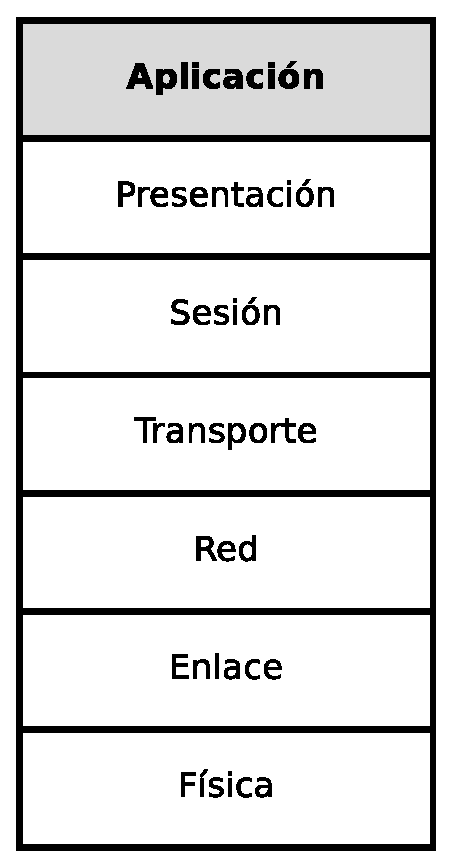
\includegraphics[width=0.25\textwidth]{img/NivelesOSI.eps}
              \caption{niveles OSI}
  \label{fig:nivelesOSI}
\end{wrapfigure}

En este proyecto se van a implementar una serie de protocolos para demostrar la versatilidad de la plataforma y sobre todo la comodidad y la limpieza de codigo que aportan. Se pretende conseguir una plataforma que facilite la implementación de servicios para protocolos a nivel de Aplicacion.

Limitando la comunicación al nivel de aplicación todos los protocolos existentes pueden resumirse como una secuencia de emisión y recepción de datos en una serie de etapas y formatos establecidos por el protocolo. 

De esta manera se puede entender al servicio como un autómata sensible al contexto para cada conexión que recibe. Orientando el diseño del servicio como una secuencia de pasos y que estos sean lo más simple y claro posible se ahorrará mucho tiempo y complejidad en la producción del codigo. 

Es dificil generalizar sobre protocolos ya que estos varian ampliamente en proposito y en complejidad. La mayoria de los protocolos de red poseen alguna de las siguiente propiedades:

\begin{enumerate}
\item Detección de la capa subyacente de enlace de red, o la existencia de otro punto de entrada o nodo.
\item Saludo y reconocimiento (Handshaking)
\item Negociación de varias de las caracteristicas de la conexión.
\item Como indicar el comienzo y el final de un mensaje.
\item Formato de los mensajes.
\item Como actuar ante mensajes corruptos o con un formato incorrecto (corrección de errores)
\item Como detectar una perdida inesperada de la conexion y como comportarse ante esta.
\item Finalizar la sesión o conexión.
\end{enumerate}

Los protocolos elegidos para demostrar la idoneidad de la plataforma son los siguientes


\section{Telnet}
Se trata de un cl\'asico obligado entre cualquier conjunto de servicios de red (o su sustituto Secure SHell). La función de este servicio consisten en proveer de autentificacion y acceso al control de las terminales de un sistema.

TELNET (TELecommunication NETwork) es un protocolo de red utilizado en conexiones de internet o en redes de area local (LAN). Fue desarrollado en 1969 y especificado en el RFC 15 y despues estandarizado en el IETF STD 8, uno de los primeros estandares de internet.

El termino telnet tambien se refiere al software que implementa a la parte cliente del protocolo. Los clientes TELNET estan disponibles en prácticamente cualquier plataforma. La mayoria de los equipos de red que dispongan de una pila TCP/IP tienen soporte  para algun tipo de servidor TELNET para permitir su configuracion remota (incluyendo a los basados en Windows NT). Debido a los problemas de privacidad con TELNET se ha reemplazado ampliamente por SSH (Secure SHell).

El termino ``hacer un telnet'' es la forma de llamar a establecer una conexión o utlizar TELNET u otras conexiones TCP interactivas. Como ejemplo: ``Para cambiar tu contraseña, haz telnet al servidor y ejecuta el comando passwd''.

Muy a menudo un usuario hará telnet a un sistema tipo Unix o a un simple dispositivo de red com un router. Por ejemplo un usuario podría ``hacer telnet desde casa para mirar su correo en el colegio''. De la misma manera podria utilizar un cliente telnet para conectar desde su equipo de escritorio con sus servidores. Una vez que la conexion, el usuario podrá ingresar con sus datos de acceso y ejecutar comandos en el sistema remoto.

En algunos sistemas el cliente se puede utilizar para realizar sesiones TCP en bruto. Comunmente se cree que una sesion telnet que no incluye un IAC (el caracter 255) tiene la misma utilidad. Esta no es el caso ya que debido a NVT (Terminales Virtuales de Red) con reglas especiales como el empleo constante de los caracteres 0 o 13.

\section{HTTP: HiperText Transfer Protocol}
Elaborado por el W3C y la IETF el HTTP es seguramente uno de los servicios de red más extendido en internet y en redes internas. Define las normas de comunicación entre los participantes del servicio (clientes, servidores y opcionalmente proxies). Servirá como ejemplo para abordar la programacion de un protocolo m\'as avanzado y permita su uso desde los diversos tipos de navegadores.

El Hypertext Transfer Protocol (HTTP) es un protocolo de comunicaciones para transferencia de informacion a trav\'es de Internet. Su utilización par recuperar documentos de texto vinculados (hipertexto) a llevado al establecimiento de la World Wide Web.

El desarrollo del HTTP fue coodinado por el Consorcio World Wide Web (W3C) y la Internet Engineering Task Force (IETF), culminando en la publicacion de una serie de RFCs, siendo el más desatacable el RFC 2616 que en Junio de 1999 definio el HTTP versión 1.1, que es la que más ampliamente se utiliza en la actualidad.

HTTP es un estandar petición/respuesta entre un cliente y un servidor. El cliente será el usuario final mientra que el servidor es el sitio web (web site). El cliente, realizando una peticion HTTP mediante un navegador web, araña web u otras herramientas, se le denomina user agent. El servidor correspondiente, que almacena o crea recursos como ficheros HTML e imagenes, es denominado servidor de origen. Entre el user agent y el servidor origen pueden aparecer varios intermediarios, como son los proxys, pasarelas y tuneles. El GTTP no esta limitado a su utilización sobre TCP/IP y sus capas, más aun es la aplicación mas extendida en Internet. Ciertamente HTTP puede implementarte sobre sobre otros protocolos en Interneto en otras redes. HTTP solo asume que se encuentra sobre un protoclo de transporte confiable, con lo que HTTP puede utilizarse sobre cualquier protocolo que lo garantice.

Normalmente es el cliente HTTP el que inicia la peticion. Se establece una conexion TCP a un puerto particular en un servidor (el puerto 80 por defecto). el servidor HTTP escuchando en ese puerto esperara a que el cliente emita el mensaje de petición. Una vez recibida la petición el servidor reponde con una linea de estado, como por ejemplo ``HTTP/1.1 200 OK'',  un mensaje propio, el cuerpo de lo que probablemente sea el fichero solicitado, mensajes de error si procede y otras informaciones.

La razón por la que HTTP se basa en TCP y no en UDP es debida a la cantidad de datos que se generan al enviar una pagina web y a que TCP provee control de transmisión, envia los datos en orden y provee corrección de errores.

Los recursos a los que se puede acceder mediante HTTP se identifican mediante Identificadores Unificados de Recursos (URIs) y en concreto Localizadores Unificador de Recursos (URLs).


\section{SIP: Session Initiation Protocol} 

Es un protocolo desarrollado por el IETF MMUSIC Working Group en la busqueda de un estandar para iniciar, finalizar o modificar sesiones interactivas de usuario, que se emplearan para contactar con dichos usuarios. Normalmente se utiliza en conjunción con otros servicios, principalmente multimedia (video, voz, mensajeria instantanea). Se ha convertido en el protocolo de señalización para voz por IP más utilizado junto al H.232.

El Session Initiation Protocol es un protocolo de señalización, ampliamente utilizado para iniciar y desconectar sesiones de comunicaciones multimedia, como llamadas de voz y video a trav\'es de internet. Otras aplicaciones interesantes incluyen conferencias de video, streaming multimedia, mensajeria instantanea, información de presencia y juegos online. En Noviembre del 2000 SIP fue adoptado como protocolo de señalización para 3GPP y elemento permanente de la arquitectura IMS para streaming multimedia sobre IP para telefonos celulares.

Este protocolo puede utilizarse para crear, modificar y finalizar sesiones unicast o multicast consistentes en uno o varios flujos de medios. La modificacion puede suponer cambiar direcciones o puertos, invitar a otros participantes, añadir o retirar flujos de medios, etc.

SIP puede situarse sobre los proctolos TCP, UDP o SCTP. Fue originariamente diseñador por Henning Schulzrinne (Universidad de Columbia) y Mark Handley (UCL) en 1996. La ultima version de la especificacion es el RFC 3261 del IETF SIP Working Group.

Cabe destacar que SIP funciona en modo texto, lo que hace más facil analizar su funcionamiento.


\chapter{Análisis}
El modelo Cliente-Servidor es tan básico como antiguo, se pueden considerar que los primeros sistemas de este tipo eran los teletipos utilizados en las universidades para emitir programas a los equipos que alli habian instalados y recibir posteriormente sus resultados. A diferencia de hoy aquellos sistemas funcionaban directamente sobre enlaces dedicados y cada uno de estos teletipos disponia de una conexión permanente.

Sin embargo la implantación de sistemas de red por capas, enlaces no dedicados y sobre todo la diversificación de equipos mucho mas baratos y potentes han modificado el panorama de manera importante: Además de diversificarse los tipos de servicios era posible que varios de ellos coexisitieran en el mismo equipo.

En el contexto de los sistemas informáticos un protocolo es un conjunto de reglas predefinidas, cuyo proposito es estandarizar actividades y procesos. Siguiendo un mismo protocolo se garantiza que se mantendrá la compatibilidad entre los sistemas involucrados, independientemente del medio sobre el que est\'en en contacto, posiblemente otros protocolos.


La forma cl\'asica de programar un servicio consiste en un blucle de escucha que inicia subprocesos para cada conexi\'on entrante y que finaliza cuando esta acaba o se produce un error. Se presentan dos entidades en este caso, la del servicio que incluiria las rutinas para iniciar la escucha y el acceso a los datos y la del manipulador, que atiende la conexion siguiendo las pautas del protocolo.
\section{Servicio}
Al arrancar un servicio antes de iniciar el bucle de escucha deben realizarse una serie de procedimientos:
\begin{enumerate}
	\item La lectura de parámetros desde linea de comandos
	\item La lectura de parámetros desde el archivo de configuracion
	\item El registro de actividad en el(los archivo(s) pertinentes
	\item Preparar el acceso a los datos necesarios, ficheros o bases de datos
\end{enumerate}

\subsubsection{parámetros}
Existen parametros que son comunes practicamente a cualquier servicio por ejemplo:
\begin{enumerate}
	\item Fichero de configuraci\'on.
	\item N\'umero de puerto para la escucha
	\item N\'umero m\'aximo de conexiones simultaneas
	\item Ficheros de registro, eventos, errores, etc
	\item Nivel de locuacidad (verbosity) en los registros.
\end{enumerate}
O parametros particulares para segun que tipos de servicio:
\begin{enumerate}
	\item Acceso al medio de datos
	\item Parametros de configuraci\'on concretos
\end{enumerate}
Debe tenerse en cuenta que los parametros en el fichero de configuracion tienen menor prevalencia que los indicados por linea de comandos, salvo el que especifique precisamente que fichero de configuracion debe leerse.

\subsubsection{Ficheros de configuración}
Debe acordarse una estructura común a todos los ficheros de configuración que se parsearán desde la plataforma pero permitiendo a la vez mantener la genericidad suficiente como para no perder la flexibilidad que haga este sistema util a cualquier implementacion de servicios y que a su vez permita que los usuarios puedan entender el fichero de forma clara y manipularlo facilmente.

Se espefican con ese fin las siguiente sintaxis:


\[<nombre parametro>=<valor>\{,<valor-N>\}\]


Para los valores que deben utilizar los parametros se pueden utilizar comodines para ampliar la versatilidad:
\begin{enumerate}
	\item \%H - Hostname
	\item \%i - Ip de la conexion entrante
	\item \%p - Puerto de origen de la conexion
	\item \%d - fecha actual
	\item \%t - hora actual
\end{enumerate}

\subsubsection{Locuacidad}
Para que puedan establecerse mensajes de depuración a distintos niveles debe adoptarse un sistema de categorias de mensajes, en cada etapa o proceso del servicio y del manipulador se emiten mensajes que incorporan el nivel de locuacidad para el que son generados, será la clase encargada de mostrar mensajes la que los muestre segun si el nivel de estos es menor o no que el indicado.
Se proponen los siguientes niveles
\begin{enumerate}
	\item 0 - Básico: mensajes de operaciones minimo, inicio del sistema, errores en los procedimientos.
	\item 1 - Moderado: mensajes comunes, entrada en servicio de un manipulador y puntos clave del desarrollo de la atención.
	\item 2 - Productivo: indica la entrada en la mayoria de las etapas de un servicio. Se amplian los detalles de los mensajes de error
	\item 3 - Expresivo: indica la entrada a cada etapa del servicio, se detalla el contexto de cada mensaje de error.
	\item 4 - Locuaz: detalla el contexto de cada etapa.
\end{enumerate}

\subsubsection{Registro}
Con la intencion de simplificar la tarea de gestionar la salida de mensajes, bien a la salida de la consola o a ficheros de registro deben implementarse clases destinadas a tal fin, que vuelquen o no los mensajes al medio según la locuacidad que se ha fijado y que en caso de que el medio predeterminado falle (por falta de espacio o cambio de permisos) sea capaz de cambiar a otro (indicado en la configuracion o a los medios salida por pantalla dedicados a tal fin).

\section{Manipulador}
Precisamente es la naturaleza de un protocolo, como un conjunto ordenado de etapas en las que se organiza el flujo de informacion entre los sistemas, la que permite abstraer al programa servidor como un automata sensible al contexto. Cada etapa del manipulador equivale al estado del automata y pueden realizarse un conjunto determinado de acciones:
\begin{enumerate}
	\item Recibir datos desde la conexión
	\item Emitir datos a la conexión
	\item Tratar, almacenar o recuperar datos
	\item Avanzar, saltar o retroceder a otra etapa
\end{enumerate}

La recepción de los datos puede además controlarse mediante expresiones regulares según las especificaciones del protocolo, detectando rapidamente errores en la entrada. Debe facilitarse además la adopción de distintos tipos de intercambio de datos, controlados, formato en bruto o encriptados para evitar reimplementaciones de esta clase de rutinas.

En el diseño del manipulador debe tenerse en cuenta que normalmente existe un orden convencional en las etapas, previsiblemente estas deberia contener un numero limitado de procedimientos, para reducir la complejidad.



\end{document}

